\documentclass[12pt,a4paper]{report}

\usepackage[utf8]{inputenc}
\usepackage[T1]{fontenc}


\usepackage[margin=3cm]{geometry}
\usepackage{tabularx}
\usepackage{booktabs}
\usepackage{graphicx}
\usepackage{hyperref}
\usepackage{pdfpages}
\usepackage{makeidx}
\usepackage{listings}
\usepackage{color}
\usepackage{xcolor}
\usepackage{indentfirst}
\usepackage{caption}
\usepackage[portuguese]{babel}
\usepackage[Bjornstrup]{fncychap}
\usepackage{graphicx}
\usepackage{pgf-umlsd}
\usepackage{float}
\newcommand*{\escape}[1]{\texttt{\textbackslash#1}}

\usepackage{enumitem}

%JSON REPRESENTATION

\usepackage{bera}% optional: just to have a nice mono-spaced font
\usepackage{listings}
\usepackage{xcolor}

\colorlet{punct}{red!60!black}
\definecolor{background}{HTML}{EEEEEE}
\definecolor{delim}{RGB}{20,105,176}
\colorlet{numb}{magenta!60!black}

\lstdefinelanguage{json}{
    basicstyle=\normalfont\ttfamily,
    numbers=left,
    numberstyle=\scriptsize,
    stepnumber=1,
    numbersep=8pt,
    showstringspaces=false,
    breaklines=true,
    frame=lines,
    backgroundcolor=\color{background},
    literate=
     *{0}{{{\color{numb}0}}}{1}
      {1}{{{\color{numb}1}}}{1}
      {2}{{{\color{numb}2}}}{1}
      {3}{{{\color{numb}3}}}{1}
      {4}{{{\color{numb}4}}}{1}
      {5}{{{\color{numb}5}}}{1}
      {6}{{{\color{numb}6}}}{1}
      {7}{{{\color{numb}7}}}{1}
      {8}{{{\color{numb}8}}}{1}
      {9}{{{\color{numb}9}}}{1}
      {:}{{{\color{punct}{:}}}}{1}
      {,}{{{\color{punct}{,}}}}{1}
      {\{}{{{\color{delim}{\{}}}}{1}
      {\}}{{{\color{delim}{\}}}}}{1}
      {[}{{{\color{delim}{[}}}}{1}
      {]}{{{\color{delim}{]}}}}{1},
}

%END JSON REPRESENTATION






\title{\mytitle}
\author{\myauthor}
\date{\mydate}

\begin{document}

\begin{titlepage} % Suppresses displaying the page number on the title page and the subsequent page counts as page 1
	\newcommand{\HRule}{\rule{\linewidth}{0.5mm}} % Defines a new command for horizontal lines, change thickness here
	
	\center % Centre everything on the page
	
	%------------------------------------------------
	%	Headings
	%------------------------------------------------
	
	\textsc{\LARGE FCT-NOVA}\\[1.5cm] % Main heading such as the name of your university/college
	
	\textsc{\Large Arquitectura e Protocolos de Redes de Computadores}\\[0.5cm] % Major heading such as course name
	
	\textsc{\large Relatório Lab. 2}\\[0.5cm] % Minor heading such as course title
	
	%------------------------------------------------
	%	Title
	%------------------------------------------------
	
	\HRule\\[0.4cm]
	
	{\huge\bfseries Passive Network Measurements and Analysis of NetFlow data}\\[0.4cm] % Title of your document
	
	\HRule\\[1.5cm]
	
	%------------------------------------------------
	%	Author(s)
	%------------------------------------------------
	
	\begin{minipage}{0.3\textwidth}
		\begin{flushleft}
			\large
			
		\end{flushleft}
	\end{minipage}
	~
	\begin{minipage}{0.6\textwidth}
		\begin{flushright}
			\large
			\textit{Autores}
			\\
			Rodrigo Faria Lopes nº 50435 %Your name
			\\
			João Machado nº 58722 %Your name
			\\
			\textit{Professores}:
			\\
			José Legatheaux Martins\\
			Paulo Afonso Lopes
			\\
			\textit{Turno}: P1
		\end{flushright}
	\end{minipage}
	
	% If you don't want a supervisor, uncomment the two lines below and comment the code above
	%{\large\textit{Author}}\\
	%John \textsc{Smith} % Your name
	
	%------------------------------------------------
	%	Date
	%------------------------------------------------
	
	\vfill\vfill\vfill % Position the date 3/4 down the remaining page
	
	{\large\today} % Date, change the \today to a set date if you want to be precise
	
	%------------------------------------------------
	%	Logo
	%------------------------------------------------
	
	\vfill\vfill
	
\includegraphics[width=0.2\textwidth]{Images/UNL.jpg}\\[1cm] % Include a department/university logo - this will require the graphicx package
	 
	%----------------------------------------------------------------------------------------
	
	\vfill % Push the date up 1/4 of the remaining page
	
\end{titlepage}
\newpage

\tableofcontents

\newpage
\chapter{Introdução}

Neste relatório iremos mostrar e explicar os resultados obtidos da análise de dois ficheiros distintos (www.fct.unl.pt.csv e bigFlows.csv) respondendo às perguntas especificadas do enunciado fornecido. Todos os tópicos foram implementados desde as obrigatórias (a1, a2, a3, a4 e a5) às opcionais (b1, e b2).

A implementação deste enunciado é escrito em código Python na sua versão 3 \cite{PYTHON3}, tendo sido também usada uma API externa e um ficheiro auxiliar, para a Geolocalização \cite{API} (IPGeolocation.py) e listagem das portas TCP e UDP \cite{PORTS} respectivamente. O uso da API requis uma autenticação, pelo que usamos as nossas contas Gmail da faculdade para obter as chaves necessárias (estando estas \textit{
harcoded} nos ficheiros necessários)

Inicialmente começamos por implementar um \textit{script} (intoDB.py) para inserir todos os dados do ficheiro .csv para uma base de dados relacional (SQLite \cite{SQLite}) de forma a mais tarde poder-mos fazer as perguntas utilizando SQL. Esta abordagem posteriormente não foi utilizada, porque achamos que talvez fosse mais confuso. Então decidimos manter o ficheiro intoDB.py para eventuais trabalhos de otimização futuros caso estes fossem necessários.

Nos tópicos opcionais (b1 e b2) optamos por criar os gráficos pretendidos utilizando a biblioteca \textit{matplotlib} \cite{MAT} de modo a converter a nossa informação em forma de mapa (key value) em gráficos 2D.

De seguida iremos, em cada capitulo, mostramos os nossos resultados para cada tópico do enunciado, falando da nossa abordagem ao problema e forma como esta foi implementada.

Inicialmente começamos por implementar uma estratégia de leitura dos ficheiros, onde abrimos o ficheiro pretendido iterando linha a linha a informação nele contida. O formato deste código foi repetido para os diferentes \textit{scripts} de modo a facilitar e dividir cada tópico pretendido.

\clearpage

Cada coluna, em termos de código, será representada da seguinte forma:
\begin{itemize}
    \item row[0] = time start
    \item row[1] = time end
    \item row[2] = duration (s)
    \item row[3] = source address
    \item row[4] = destination address
    \item row[5] = source port
    \item row[6] = destination port
    \item row[7] = protocol
    \item row[8] = flags
    \item row[9] = packets
    \item row[10] = bytes
\end{itemize}

Na figura 1.1 podemos ver esta parte do \textit{script} comum a todos os ficheiros implementados, não sendo esta mais falava nos próximos capítulos por motivos de repetição:

\begin{figure}[h]
    \label{high}
    \centering
    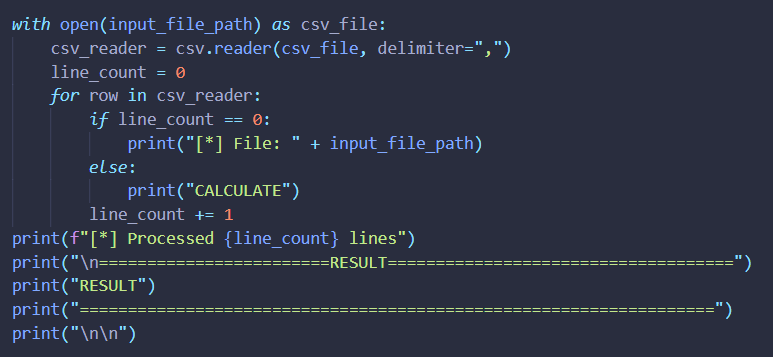
\includegraphics[width=1\textwidth]{Images/reader.png}
    \caption{\textit{Código inicial para cada tópico}}
\end{figure}

\textbf{Nota:} O código está num repositório GitHub privado, pelo que caso queira ter acesso ao mesmo deverá enviar um email aos autores a pedir autorização de acesso.

Link: \textbf{\url{https://github.com/rfa-lopes/APRC}}
\chapter{A1}

{\LARGE 'Compute the total number of packets and bytes (in and out) per protocol (TCP, UDP, ICMP, …) contained in the flows.'}

\section{Explicação do código desenvolvido}

A computação deste tópico foi relativamente fácil, onde apenas foi necessário iterar todos os tuplos do ficheiro, verificar o seu protocolo e adicionar a uma mapa o eu número de \textit{bytes} e \textit{packets}. Como já foi referido, neste tópico utilizamos uma estrutura de dados \textit{(Key, Value)} para guardar em memória os resultados de cada iteração. O código seguinte mostra a parte do \textit{script} que trata de cada tuplo do ficheiro.

\begin{figure}[h]
    \label{high}
    \centering
    
\includegraphics[width=1\textwidth]{Images/a1/a1.png}
    \caption{\textit{Código do tópico a1}}
\end{figure}

%----------------------------------------------------------------------------
%----------------------------------------------------------------------------

\clearpage

\section{Resulados obtidos pelo ficheiro www.fct.unl.pt.csv}

Como se pode ver na figura 2.2, foram processadas as 21362 linhas do ficheiro www.fct.unl.pt.csv, existindo fluxos TCP, UDP e ICMP, estando associados a cada um destes o número de \textit{bytes} e \textit{packets} como pretendido.

\begin{figure}[h]
    \label{high}
    \centering
    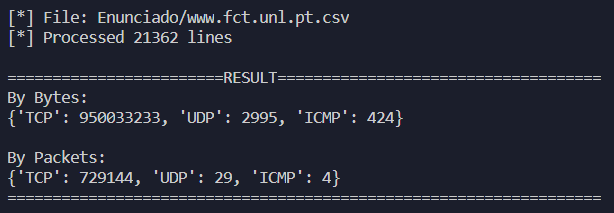
\includegraphics[width=1\textwidth]{Images/a1/a1_a.png}
    \caption{\textit{Output do script a1.py}}
\end{figure}

%----------------------------------------------------------------------------

\section{Resulados obtidos pelo ficheiro bigFlows.csv}

Na figura 2.3 verificamos a mesma estrutura de resultados mas agora para o ficheiro bigFlows.csv, onde podemos verificar que este apresenta um tipo de protocolo que não existia no ficheiro anterior, IGMP.

\begin{figure}[h]
    \label{high}
    \centering
    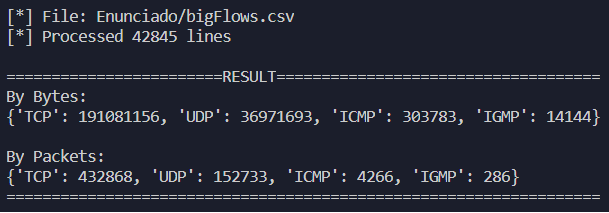
\includegraphics[width=1\textwidth]{Images/a1/a1_b.png}
    \caption{\textit{Output do script a1.py}}
\end{figure}
\chapter{A2}

{\LARGE 'Determine the 50 most popular IP addresses external to the domain by number of flows'}
´
\section{Explicação do código desenvolvido}

A computação deste tópico não apresentou uma dificuldade muito superior em comparação com o tópico anterior, no entanto foi usada uma função auxiliar para facilitar e tornar o código mais legível. A função auxiliar basicamente diz-nos se o endereço IP que estamos a tratar faz parte do domínio ou se é externo. Assim conseguimos com facilidade fazer uma lsita de tuplos onde agrupamos o \textit{IP} com o número de \textit{flows}. Por fim fazemos uma ordenação pela quantidade de flows e descartamos quaisquer resultados após os 50 primeiros. O código seguinte mostra a parte do \textit{script} que trata de cada tuplo do ficheiro.


%TODO
\begin{figure}[h!]
    \label{high}
    \centering
    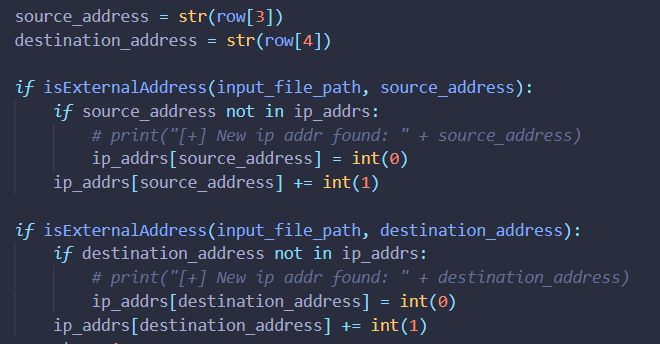
\includegraphics[width=0.8\textwidth]{Images/a2/a2.png}
    \caption{\textit{Código do tópico a2}}
\end{figure}

%----------------------------------------------------------------------------
%----------------------------------------------------------------------------

\newpage

\section{Resulados obtidos pelo ficheiro www.fct.unl.pt.csv}

Como  se  pode  ver  na  figura  3.3,  foram  processadas  as  21362  linhas  do ficheiro www.fct.unl.pt.csv, e foram recolhidos e ordenados os endereços IPs com maior número de flows.

\begin{figure}[h]
    \label{high}
    \centering
    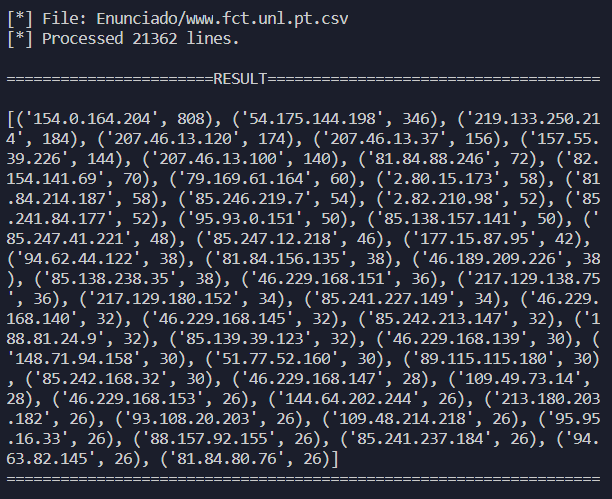
\includegraphics[width=0.9\textwidth]{Images/a2/a2_a.png}
    \caption{\textit{Output do script a2.py}}
\end{figure}

\newpage

%----------------------------------------------------------------------------

\section{Resulados obtidos pelo ficheiro bigFlows.csv}

Na figura 3.4 verificamos que foram processadas 42845 linhas do ficheiro bigFlows.csv, e foram recolhidos e ordenados os endereços IPs com maior número de flows. Fique de notar a diferença na quantidade de flows recolhida.

\begin{figure}[h]
    \label{high}
    \centering
    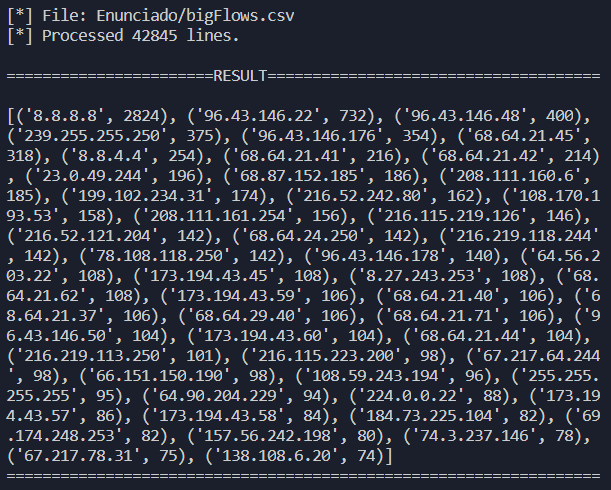
\includegraphics[width=1\textwidth]{Images/a2/a2_b.png}
    \caption{\textit{Output do script a2.py}}
\end{figure}

\chapter{A3}

{\LARGE 'Determine the 50 most popular IP addresses external to the domain by number of bytes.'}

\section{Explicação do código desenvolvido}

Se compararmos com os outros códigos, a computação deste talvez seja considerada a mais simples. Isto não pela sua complexidade por si só, mas pela semelhança com o código em A2. No fundo, a única entre os dois devesse só a onde, nos ficheiros csv, ir buscar o resultado. Observe-se no código abaixo, que os \textit{bytes} são conseguidos na coluna 10 do ficheiro.

\begin{figure}[h!]
    \label{high}
    \centering
    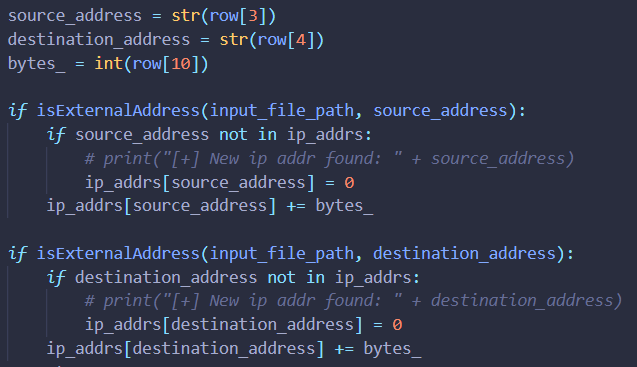
\includegraphics[width=0.9\textwidth]{Images/a3/a3.png}
    \caption{\textit{Código do tópico a3}}
\end{figure}

%----------------------------------------------------------------------------
%----------------------------------------------------------------------------

\newpage

\section{Resultados obtidos pelo ficheiro www.fct.unl.pt.csv}

Como  se  pode  ver  na  figura  4.3,  foram  processadas  as  linhas do ficheiro www.fct.unl.pt.csv, tendo ordenado, por número de bytes, os endereços IP.

\begin{figure}[h]
    \label{high}
    \centering
    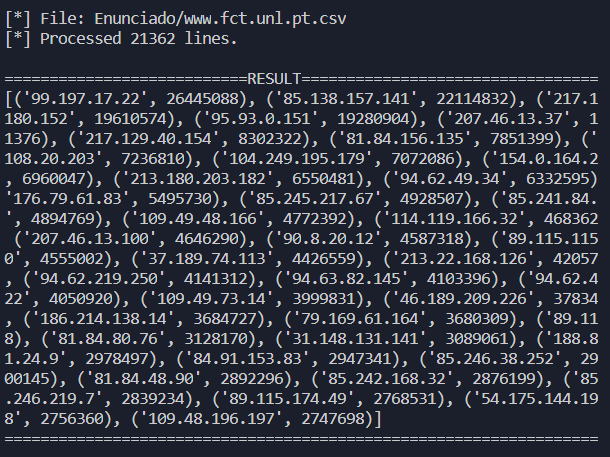
\includegraphics[width=1\textwidth]{Images/a3/a3_a.png}
    \caption{\textit{Output do script a3.py}}
\end{figure}

%----------------------------------------------------------------------------

\section{Resultados obtidos pelo ficheiro bigFlows.csv}

Como  se  pode  ver  na  figura  4.4,  foram  processadas  as  linhas do ficheiro bigFlows.csv, tendo ordenado, por número de bytes, os endereços IP.

\begin{figure}[h]
    \label{high}
    \centering
    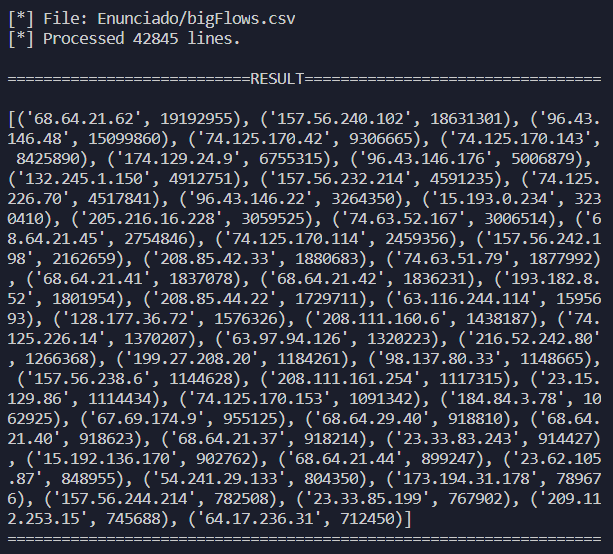
\includegraphics[width=1\textwidth]{Images/a3/a3_b.png}
    \caption{\textit{Output do script a3.py}}
\end{figure}
\par
Este exercício foi realizado de forma quase igual ao anterior, sendo a única diferença que em vez de nos vermos o flow, vimos o número de bytes como foi pedido.
\chapter{A4}

{\LARGE 'What are the top 50 most popular applications used by the computers in the domain?'}

\textbf{Nota:} There is a Wikipedia page that lists the assigned port numbers, https://en.wikipedia.org/wiki/List\_of\_TCP\_and\_UDP\_port\_numbers. Or you can Google for the IANA’s Well Known Port Numbers.

\section{Explicação do código desenvolvido}

A computação deste tópico já trouxe mais dificuldades, não propriamente no conseguir os resultados, mas em trata-los de forma a ter um output compreensível e legível. No excerto de código abaixo, mostramos que fomos simplesmente buscar os dados que nos interessavam, ou seja \textit{Source Port, Destination Port e Packets}, às colunas correspondentes do ficheiro bigFlows.csv.

\begin{figure}[h!]
    \label{high}
    \centering
    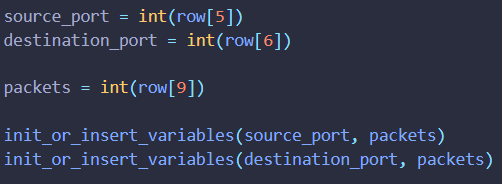
\includegraphics[width=0.9\textwidth]{Images/a4/a4.png}
    \caption{\textit{Código do tópico a4}}
\end{figure}

\newpage

É neste excerto de código que fazemos o tratamento de dados de forma semelhante aos tópicos anteriores.

\begin{figure}[h!]
    \label{high}
    \centering
    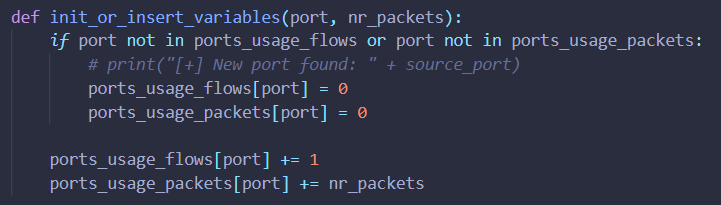
\includegraphics[width=0.9\textwidth]{Images/a4/initOrInsertVariables.png}
    \caption{\textit{Código auxiliar do tópico a4}}
\end{figure}

E para termos um output compreensível usamos as seguintes funções auxiliares. A primeira dá-nos um mapa onde cada por corresponde um uma aplicação, como exemplo temos o \textit{port 80} que corresponde a \textit{Hypertext Transfer Protocol (http)}. A segunda "pega" nos ports dos nossos resultados e atribui-lhes um nome baseado nesse mapa, como exemplo se tivermos um \textit{port 443} nos nossos resultados, esta função atribui-lhe o nome https como está no mapa.

\begin{figure}[h!]
    \label{high}
    \centering
    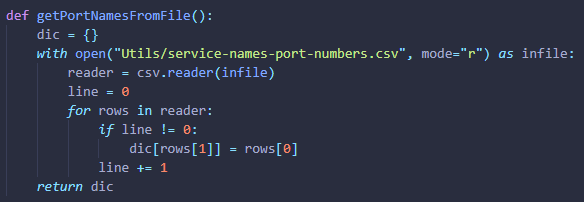
\includegraphics[width=0.9\textwidth]{Images/a4/getPortNamesFromFile.png}
    \caption{\textit{Código auxiliar do tópico a4}}
\end{figure}

\begin{figure}[h!]
    \label{high}
    \centering
    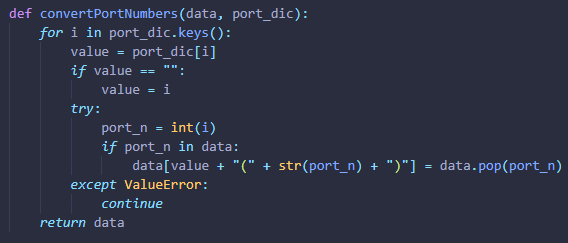
\includegraphics[width=0.9\textwidth]{Images/a4/convertPortNumbers.png}
    \caption{\textit{Código auxiliar do tópico a4}}
\end{figure}

\newpage


\section{Resultados obtidos pelo ficheiro bigFlows.csv}

No enunciado do trabalho é nos perguntado se somos surpreendidos pelo resultado. A resposta é sim e não. Foi surpreendente a quantidade de ports que obtivemos que não tiveram nenhum mapeamento aos ports da lista que usamos, sendo que nem todos são de aplicações externas (ports 49152 a 65535). No entanto, dos ports que conseguimos identificar, já esperávamos quais é que teriam mais fluxo.

\begin{figure}[h]
    \label{high}
    \centering
    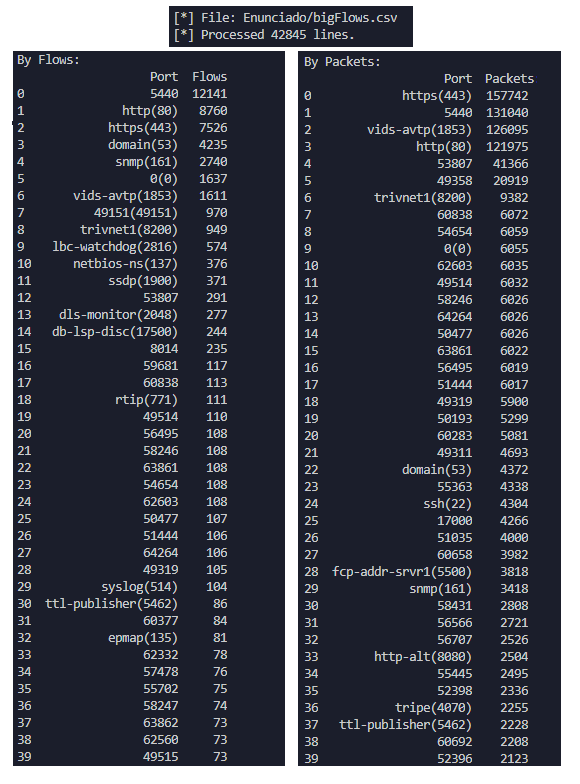
\includegraphics[width=0.85\textwidth]{Images/a4/a4_a.png}
    \caption{\textit{Output do script a4.py}}
\end{figure}


\chapter{A5}

{\LARGE 'Aggregate the two flows representing the same TCP connection; count the total number of TCP connections collected, and the total number of TCP connections that started and finished correctly.'}

\section{Explicação do código desenvolvido}

Este código foi sem dúvida alguma o mais complicado da parte "mandataria". Foi complicado não só codificar mas também perceber o pedido para poder começar a construí-lo. Usámos a mesma estratégia para obter os dados usada previamente. Feito isso precisámos de garantir que o que quer que fizéssemos fosse apenas sobre uma única conexão TCP, daí o \textit{if} que verifica se duas linhas correspondem a mesma conexão. Aí precisámos de saber se a conexão tinha começado e acabado com sucesso. Para fazer isso tivemos que usar as \textit{flags} e concluímos que uma conexão iniciada com sucesso necessita das \textit{flags} \textit{ACK} e \textit{SYN}, e uma conexão terminada com sucesso necessita da \textit{flag} \textit{F}.

\begin{figure}[h!]
    \label{high}
    \centering
    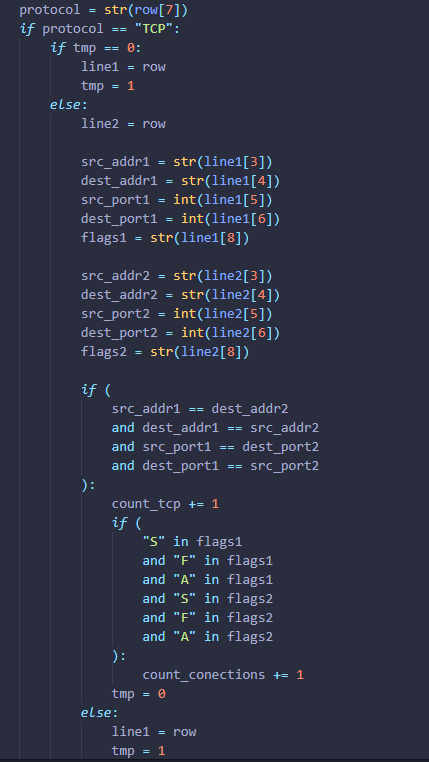
\includegraphics[width=0.8\textwidth]{Images/a5/a5.png}
    \caption{\textit{Código do tópico a5}}
\end{figure}

%----------------------------------------------------------------------------
%----------------------------------------------------------------------------
\clearpage

\section{Resulados obtidos pelo ficheiro www.fct.unl.pt.csv}

Como se pode ver na figura 6.2, foram processadas as linhas do ficheiro www.fct.unl.pt.csv. Apresentamos no output o total de conexões TCP e quantos dessas começaram e terminaram com sucesso.

\begin{figure}[h]
    \label{high}
    \centering
    
\includegraphics[width=1\textwidth]{Images/a5/a5_a.png}
    \caption{\textit{Output do script a5.py}}
\end{figure}

%----------------------------------------------------------------------------

\section{Resulados obtidos pelo ficheiro bigFlows.csv}

Como se pode ver na figura 6.3, foram processadas as linhas do ficheiro bigFlows.csv. Apresentamos no output o total de conexões TCP e quantos dessas começaram e terminaram com sucesso.

\begin{figure}[h!]
    \label{high}
    \centering
    
\includegraphics[width=1\textwidth]{Images/a5/a5_b.png}
    \caption{\textit{Output do script a5.py}}
\end{figure}

%----------------------------------------------------------------------------

\clearpage

\section{'Explain the several possible technical reasons that justify why there are TCP connections that were not started or ended correctly.'}

Problemas no inicio das conexões, SYN+ACK.
A conexão está a ser largada em algum sitio durante o envio, geralmente por sistemas intermédios como a \textit{firewall} ou o \textit{load-balancer}. 
Também pode ser algo tão simples como um problema de \textit{routing}.

Problemas no fim da conexões, FIN.
Terminações anormais de conexões podem dever-se a:
\begin{itemize}
    \item Falta de recursos ou interrupção de \textit{internet}.
    \item Uma quebra ou um \textit{bug} na sessão.
    \item Quando um lado da conexão já terminou e fechou a mesma, mas o outro lado continua a enviar dados.
    \item O servidor recusa-se a abrir conexões com o cliente.
\end{itemize}
\chapter{B1}

{\LARGE 'Provide two charts representing the average bit rate per time unit that crossed the interface or the router in and out during the collecting period.'}

\section{Explicação do código desenvolvido}

A nossa abordagem para este problema foi tentar arranjar uma solução escalável para qualquer tipo de unidades de tempo, dado que para um ficheiro seria uma unidade de tempo de um minuto e outro com 5 segundos. 

Implementamos então duas funções auxiliares para nos ajudar na recolha desta informação. Na figura 7.1 vemos a função \textit{getTimeDiffInSecound(start, to)} onde dado um tempo inicial (start) e um tempo final (to), a função calcula a diferença em segundos desses tempos. 

A função seguinte \textit{getTimeFrameInSecound(file)} recebe um nome de um ficheiro e devolve a unidade de tempo, em segundos, que se pretende. Com esta arquitectura podemos acrescentar livremente novos ficheiros ou mesmo modificar os tempos de cada ficheiro sem ter que se modificar o código base da função b1. O resultado desta função é guardado na variável \textit{timeFrame}.

\begin{figure}[h!]
    \label{high}
    \centering
    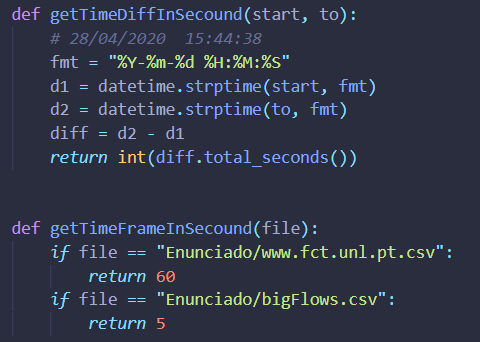
\includegraphics[width=0.6\textwidth]{Images/b1/auxFunctions.png}
    \caption{\textit{Funções auxiliares de b1}}
\end{figure}

Passando agora à explicação do código base da recolha de informação dos ficheiros, começamos por verificar o para cada tuplo (linha) o seu \textit{start\_time\_} (a variável \textit{end\_time\_} não é utilizada), que é o tempo inicial do fluxo que se encontra na primeira coluna dos ficheiros. Posteriormente incializamos a variavel \textit{start\_time} (diferente de \textit{start\_time\_}) que será o tempo inicial do primeiro bloco de tempo a ser analizado. 

A partir dai comparamos esse resultado ao \textit{start\_time\_} de cada fluxo de modo a saber se já passou o tempo necessário para passar para o próximo bloco de tempo. Quando isso acontecer, passamos ao próximo bloco de tempo (counter += 1) e dizemos que agora o \textit{start\_time} agora é o \textit{start\_time\_} do primeiro fluxo do próximo bloco de tempo.

Durante cada bloco inicializamos a nossa estrutura de dados sempre que necessário e adicionamos a ela a informação necessária caso (como requerido pelo enunciado) os IP's sejam externos, utilizando a função \textit{isExternalAddress(file, address)} já explicada nos capítulos anteriores.

\begin{figure}[h!]
    \label{high}
    \centering
    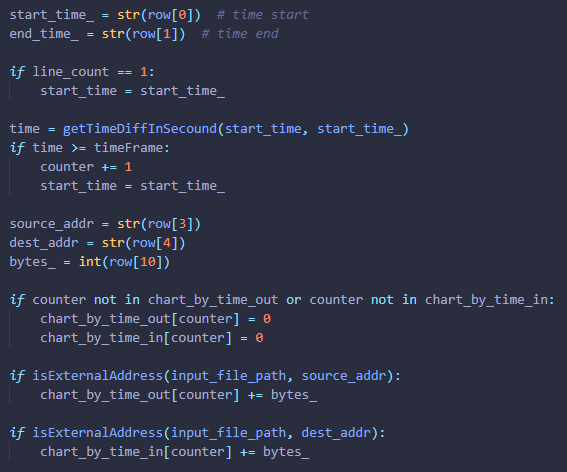
\includegraphics[width=0.9\textwidth]{Images/b1/b1.png}
    \caption{\textit{Código do tópico b1}}
\end{figure}

%----------------------------------------------------------------------------
%----------------------------------------------------------------------------
\newpage

\section{Resultados obtidos pelo ficheiro www.fct.unl.pt.csv}

Os resultados seguintes são o \textit{output} do \textit{byte rate} IN e OUT proposto por intervalos de tempo. Onde o tempo 0 para o ficheiro www.fct.unl.pt.csv equivale ao intervalo de tempo 2020-04-28 14:42:57 -> 2020-04-28 14:43:57 e o tempo 55 (último) equivale ao intervalo de tempo 28/04/2020 15:43:40 -> 28/04/2020 15:44:40, equivalente aos períodos do ficheiro.

\begin{figure}[h!]
    \label{high}
    \centering
    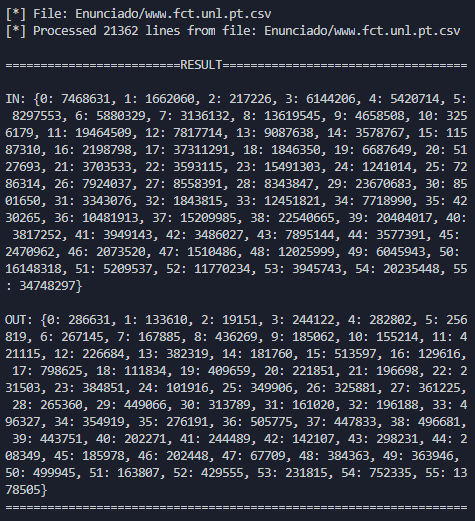
\includegraphics[width=1\textwidth]{Images/b1/b1_a.png}
    \caption{\textit{Output do script b1.py}}
\end{figure}

Utilizando a biblioteca \textit{matplotlib} \cite{MAT} foi-nos possível e tempo de execução do código mostrar um gráfico visual dos dados da figura 7.3.

\begin{figure}[h!]
    \label{high}
    \centering
    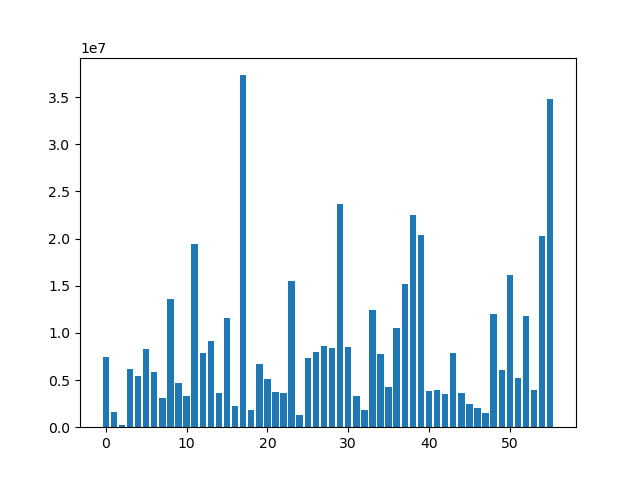
\includegraphics[width=0.9\textwidth]{Images/b1/b1_1.png}
    \caption{\textit{Gráfico do fluxo médio de bytes de entrada}}
\end{figure}

\begin{figure}[h!]
    \label{high}
    \centering
    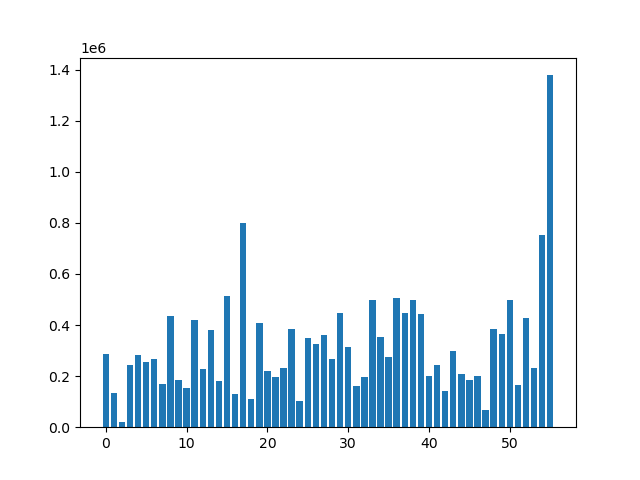
\includegraphics[width=0.9\textwidth]{Images/b1/b1_2.png}
    \caption{\textit{Gráfico do fluxo médio de bytes de saída}}
\end{figure}

\newpage

\section{Resultados obtidos pelo ficheiro bigFlows.csv}

Os resultados seguintes são o \textit{output} do \textit{byte rate} IN e OUT proposto por intervalos de tempo. Onde o tempo 0 para o ficheiro bigFlows.csv equivale ao intervalo de tempo 26/03/2020 20:27:35 -> 26/03/2020 20:27:40 e o tempo 56 (último) equivale ao intervalo de tempo 26/03/2020 20:32:30 -> 26/03/2020 20:32:35, equivalente aos períodos do ficheiro.

\begin{figure}[h!]
    \label{high}
    \centering
    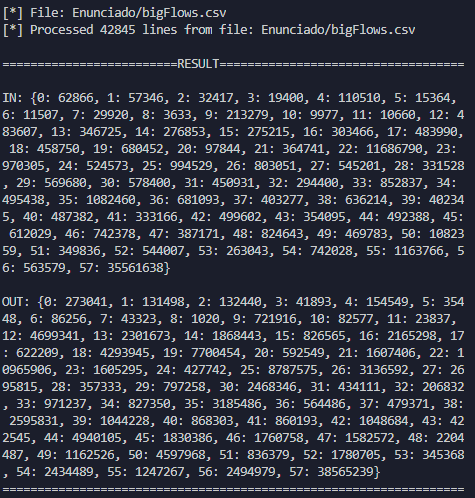
\includegraphics[width=1\textwidth]{Images/b1/b1_b.png}
    \caption{\textit{Output do script b1.py}}
\end{figure}

Utilizando a biblioteca \textit{matplotlib} \cite{MAT} foi-nos possível e tempo de execução do código mostrar um gráfico visual dos dados da figura 7.6.

\begin{figure}[h!]
    \label{high}
    \centering
    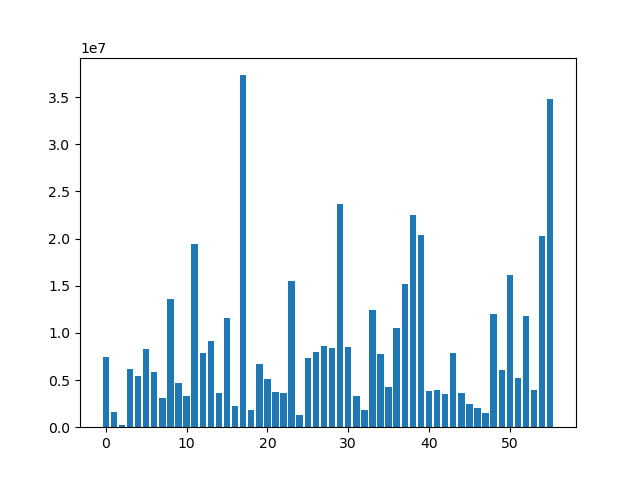
\includegraphics[width=0.9\textwidth]{Images/b1/b1_1.png}
    \caption{\textit{Gráfico do fluxo médio de bytes de entrada}}
\end{figure}

\begin{figure}[h!]
    \label{high}
    \centering
    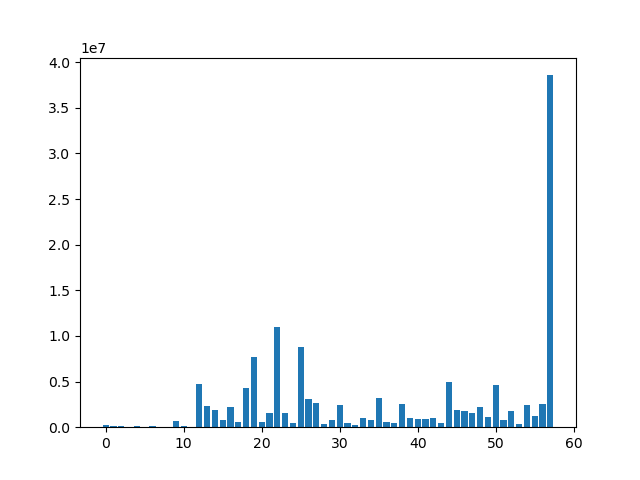
\includegraphics[width=0.9\textwidth]{Images/b1/b1_4.png}
    \caption{\textit{Gráfico do fluxo médio de bytes de saída}}
\end{figure}

\chapter{B2}

{\LARGE Consider the two files and represent in a 2D chart the geographic position of the IP addresses outside the domain computed in a.3.}

\section{Explicação do código desenvolvido}

Para o desenvolvimento deste tópico decidimos utilizar a API de Geolocalização \cite{API} que nos forneceu algum código (IPGeolocation.py) de modo a facilitar a sua utilização. Na figura 8.1 pode-se ver o código criado por nós para a conversão dos IP's por localização geográfica. 

Dado que a API só nos deixava utilizar alguns recursos por dia, fomos obrigados a utilizar duas contas para gerar duas chaves de modo a cobrir o nosso código com o maior número de testes possível. Esta função \textit{getGeoLocation(ips\_addrs)} recebe um conjunto de IP's (já computados previamente) e converte-os para uma localização geográfica. Utilizamos mais uma vez um mapa para sabermos quantas vezes aparecem IP's de uma dada localização, sendo este mapa no fim ordenado da localidade mais utilizada, para a menos utilizada.


\begin{figure}[h!]
    \label{high}
    \centering
    
\includegraphics[width=0.7\textwidth]{Images/b2/getGeoLocation.png}
    \caption{\textit{Código do tópico b2}}
\end{figure}

Na figura 8.2 podemos verificar como esta função é utilizada depois da computação dos IP's e a forma como essa informação é ordenada.

\begin{figure}[h!]
    \label{high}
    \centering
    
\includegraphics[width=0.7\textwidth]{Images/b2/result.png}
    \caption{\textit{\textit{Print} e gráfico do resultado b2}}
\end{figure}

Passando agora à analise do código que itera todas as linhas do ficheiro, podemos verificar que o código é muito simples de se entender. Inicialmente inicializamos as variáveis úteis, e caso se trate de um fluxo exterior (de origem ou destino) inicializamos a nossa estrutura de dados (mapa) e adicionamos o IP's associado. 

\begin{figure}[h!]
    \label{high}
    \centering
    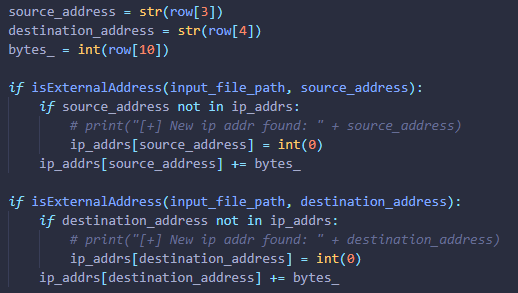
\includegraphics[width=0.9\textwidth]{Images/b2/b2.png}
    \caption{\textit{Código do tópico b2}}
\end{figure}

%----------------------------------------------------------------------------
%----------------------------------------------------------------------------
\newpage

\section{Resultados obtidos pelo ficheiro www.fct.unl.pt.csv}

Para os resultados do ficheiro www.fct.unl.pt.csv era de esperar que Portugal dominasse como localização mais comum entre os IP's. Nas figuras 8.4 e 8.5 podemos ver os resultados em forma de gráfico e em forma de mapa. 

\begin{figure}[h!]
    \label{high}
    \centering
    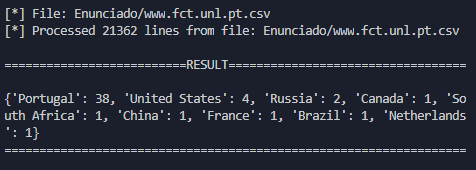
\includegraphics[width=1\textwidth]{Images/b2/b2_a.png}
    \caption{\textit{Output do script b2.py}}
\end{figure}

\begin{figure}[h!]
    \label{high}
    \centering
    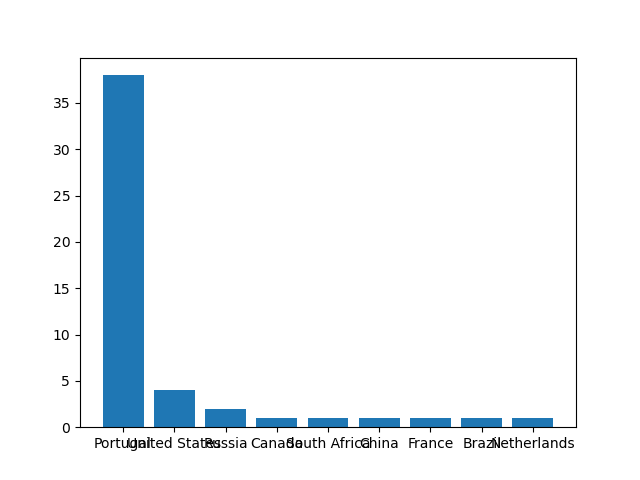
\includegraphics[width=1\textwidth]{Images/b2/b2_1.png}
    \caption{\textit{Gráfico das posições geográficas do endereços IP}}
\end{figure}

\clearpage

\section{Resultados obtidos pelo ficheiro bigFlows.csv}

Para os resultados do ficheiro bigFlows.csv os Estados Unidos dominam consideravelmente, estando os resultados apresentados nas figuras 8.6 e 8.7 seguintes.

\begin{figure}[h!]
    \label{high}
    \centering
    
\includegraphics[width=1\textwidth]{Images/b2/b2_b.png}
    \caption{\textit{Output do script b2.py}}
\end{figure}

\begin{figure}[h!]
    \label{high}
    \centering
    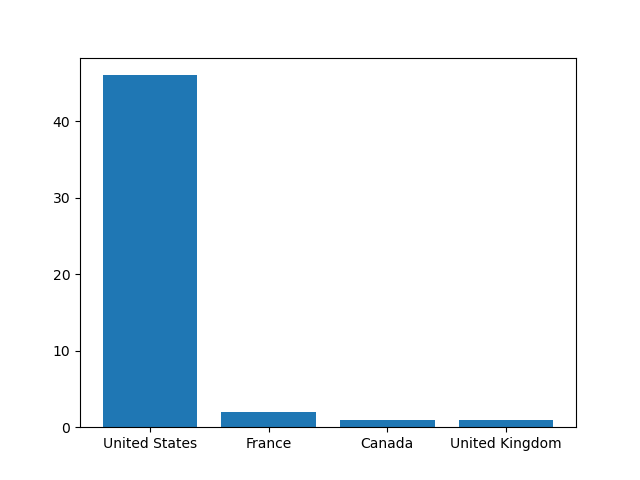
\includegraphics[width=1\textwidth]{Images/b2/b2_2.png}
    \caption{\textit{Gráfico das posições geográficas do endereços IP}}
\end{figure}
\chapter{Conclusão}

Para concluir, todos os tópicos foram concluídos com sucesso e explicados da melhor forma possível. Houve por parte dos alunos uma nova aprendizagem mais profunda da linguagem \textit{Python} assim como uma nova aprendizagem de como filtrar e ler informações sobre uma recolha de pacotes de uma rede. Achamos que os resultados poderiam ter sido analisados de uma forma mais óptima se fosse usada uma base de dados e posteriormente feitas as perguntas dos tópicos, mas em termos de tempo foi mais rápido implementar uma procura linear de complexidade 0(n) sobre os ficheiros fornecidos.
\begin{thebibliography}{9}

\bibitem{PYTHON3}
https://www.python.org/download/releases/3.0/

\bibitem{API}
https://github.com/IPGeolocation/ip-geolocation-api-python-sdk
https://api.ipgeolocation.io/

\bibitem{PORTS}
https://www.iana.org/assignments/service-names-port-numbers/service-names-port-numbers.xhtml

\bibitem{SQLite}
https://www.sqlite.org/index.html

\bibitem{MAT}
https://matplotlib.org/

\end{thebibliography}´
\appendix
\chapter{A1-Anexos}
\begin{lstlisting}
import csv

def a1(input_file_path):

    protocols_bytes = {}
    protocols_packets = {}

    with open(input_file_path) as csv_file:
        csv_reader = csv.reader(csv_file, delimiter=",")
        line_count = 0
        for row in csv_reader:
            if line_count == 0:
                print("[*] File: " + input_file_path)
            else:
                protocol = row[7]
                packets = row[9]
                bytes_ = row[10]

                if (protocol not in protocols_bytes 
                    or protocol not in protocols_packets):
                    
                    # print("[+] New protocol found: " + str(protocol))
                    protocols_bytes[str(protocol)] = int(0)
                    protocols_packets[str(protocol)] = int(0)

                protocols_bytes[str(protocol)] += int(bytes_)
                protocols_packets[str(protocol)] += int(packets)
            line_count += 1
    print(f"[*] Processed {line_count} lines")
    print("\n=====RESULT======")
    print("By Bytes:")
    print(protocols_bytes)
    print("\nBy Packets:")
    print(protocols_packets)
    print("===================")
    print("\n\n")

def main():
    print("\n\n")
    print(
        "[Compute the total number of packets and bytes (in and out) per"
        +" protocol (TCP, UDP, ICMP, …) contained in the flows.]\n"
    )
    a1("Enunciado/www.fct.unl.pt.csv")
    a1("Enunciado/bigFlows.csv")

if __name__ == "__main__":
    main()

\end{lstlisting}


\chapter{A2-Anexos}
\begin{lstlisting}
import csv


def a2(input_file_path):

    ip_addrs = {}

    with open(input_file_path) as csv_file:
        csv_reader = csv.reader(csv_file, delimiter=",")
        line_count = 0
        for row in csv_reader:
            if line_count == 0:
                print("[*] File: " + input_file_path)
            else:
                source_address = str(row[3])
                destination_address = str(row[4])

                if isExternalAddress(input_file_path, source_address):
                    if source_address not in ip_addrs:
                        # print("[+] New ip addr found: " + source_address)
                        ip_addrs[source_address] = int(0)
                    ip_addrs[source_address] += int(1)

                if isExternalAddress(input_file_path, destination_address):
                    if destination_address not in ip_addrs:
                        # print("[+] New ip addr found: " 
                        #+ destination_address)
                        ip_addrs[destination_address] = int(0)
                    ip_addrs[destination_address] += int(1)
            line_count += 1
    print(f"[*] Processed {line_count} lines.")
    print("\n======RESULT=============")
    print(sorted(ip_addrs.items(), key=lambda x: x[1], reverse=True)[0:50])
    print("===========================")
    print("\n\n")


def isExternalAddress(file, address):
    if file == "Enunciado/www.fct.unl.pt.csv":
        if address != "193.136.126.43" and address.split(".")[0] != "10":
            return True

    if file == "Enunciado/bigFlows.csv":
        addr_split = address.split(".")
        if addr_split[0] != "172" and (
            addr_split[1] != "16" or addr_split[1] != "31"):
            return True
    return False


def main():

    print("\n\n")
    print(
        "[Determine the 50 most popular IP addresses external"
        + " to the domain by number of flows..]\n"
    )
    a2("Enunciado/www.fct.unl.pt.csv")
    a2("Enunciado/bigFlows.csv")


if __name__ == "__main__":
    main()

\end{lstlisting}

\chapter{A3-Anexos}
\begin{lstlisting}
import csv


def a3(input_file_path):

    ip_addrs = {}

    with open(input_file_path) as csv_file:
        csv_reader = csv.reader(csv_file, delimiter=",")
        line_count = 0
        for row in csv_reader:
            if line_count == 0:
                print("[*] File: " + input_file_path)
            else:
                source_address = str(row[3])
                destination_address = str(row[4])
                bytes_ = int(row[10])

                if isExternalAddress(input_file_path, source_address):
                    if source_address not in ip_addrs:
                        # print("[+] New ip addr found: " + source_address)
                        ip_addrs[source_address] = 0
                    ip_addrs[source_address] += bytes_

                if isExternalAddress(input_file_path, destination_address):
                    if destination_address not in ip_addrs:
                        # print("[+] New ip addr found: "
                        #+ destination_address)
                        ip_addrs[destination_address] = 0
                    ip_addrs[destination_address] += bytes_
            line_count += 1
    print(f"[*] Processed {line_count} lines.")
    print("\n========RESULT=============")
    print(sorted(ip_addrs.items(), key=lambda x: x[1], reverse=True)[0:50])
    print("=============================")
    print("\n\n")


def isExternalAddress(file, address):
    if file == "Enunciado/www.fct.unl.pt.csv":
        if address != "193.136.126.43" and address.split(".")[0] != "10":
            return True

    if file == "Enunciado/bigFlows.csv":
        addr_split = address.split(".")
        if addr_split[0] != "172" and (
            addr_split[1] != "16" or addr_split[1] != "31"):
            return True
    return False


def main():
    print("\n\n")
    print(
        "[Determine the 50 most popular IP addresses external"
        + " to the domain by number of bytes.]\n"
    )
    a3("Enunciado/www.fct.unl.pt.csv")
    a3("Enunciado/bigFlows.csv")


if __name__ == "__main__":
    main()

\end{lstlisting}

\chapter{A4-Anexos}
\begin{lstlisting}
import csv
import pandas as pd


def a4(input_file_path, port_dic):

    ports_usage_flows = {}
    ports_usage_packets = {}

    def init_or_insert_variables(port, nr_packets):
        if port not in ports_usage_flows or port not in ports_usage_packets:
            # print("[+] New port found: " + source_port)
            ports_usage_flows[port] = 0
            ports_usage_packets[port] = 0

        ports_usage_flows[port] += 1
        ports_usage_packets[port] += nr_packets

    with open(input_file_path) as csv_file:
        csv_reader = csv.reader(csv_file, delimiter=",")
        line_count = 0
        for row in csv_reader:
            if line_count == 0:
                print("[*] File: " + input_file_path)
            else:
                source_port = int(row[5])
                destination_port = int(row[6])

                packets = int(row[9])

                init_or_insert_variables(source_port, packets)
                init_or_insert_variables(destination_port, packets)

            line_count += 1
    print(f"[*] Processed {line_count} lines.")

    dataFlows = sort_to_key_value(
        convertPortNumbers(ports_usage_flows, port_dic))
    dataPackets = sort_to_key_value(
        convertPortNumbers(ports_usage_packets, port_dic))

    print("\n======RESULT=========")
    print("By Flows:")
    print(pd.DataFrame(dataFlows.items(), columns=["Port", "Flows"]))

    print("\nBy Packets:")
    print(pd.DataFrame(dataPackets.items(), columns=["Port", "Packets"]))
    print("======================")
    print("\n\n")


def sort_to_key_value(data):
    return {
        k: v
        for k, v in sorted(data.items(), 
            key=lambda item: item[1], reverse=True)[0:50]
    }


def convertPortNumbers(data, port_dic):
    for i in port_dic.keys():
        value = port_dic[i]
        if value == "":
            value = i
        try:
            port_n = int(i)
            if port_n in data:
                data[value + "(" + str(port_n) + ")"] = data.pop(port_n)
        except ValueError:
            continue
    return data


def getPortNamesFromFile():
    dic = {}
    with open("Utils/service-names-port-numbers.csv", mode="r") as infile:
        reader = csv.reader(infile)
        line = 0
        for rows in reader:
            if line != 0:
                dic[rows[1]] = rows[0]
            line += 1
    return dic


def main():
    print("\n\n")
    print(
        "[What are the top 50 (or less if their variety "
        + "is smaller) most popular "
        + "applications used by the computers in the domain?]\n"
    )
    # Only for the bigFlows.csv file:
    a4("Enunciado/bigFlows.csv", getPortNamesFromFile())


if __name__ == "__main__":
    main()

\end{lstlisting}

\chapter{A5-Anexos}
\begin{lstlisting}
import csv


def a5(input_file_path):

    count_tcp = 0
    count_conections = 0

    line1 = {}
    line2 = {}
    tmp = 0

    with open(input_file_path) as csv_file:
        csv_reader = csv.reader(csv_file, delimiter=",")
        line_count = 0
        for row in csv_reader:
            if line_count == 0:
                print("[*] File: " + input_file_path)
            else:
                protocol = str(row[7])
                if protocol == "TCP":
                    if tmp == 0:
                        line1 = row
                        tmp = 1
                    else:
                        line2 = row

                        src_addr1 = str(line1[3])
                        dest_addr1 = str(line1[4])
                        src_port1 = int(line1[5])
                        dest_port1 = int(line1[6])
                        flags1 = str(line1[8])

                        src_addr2 = str(line2[3])
                        dest_addr2 = str(line2[4])
                        src_port2 = int(line2[5])
                        dest_port2 = int(line2[6])
                        flags2 = str(line2[8])

                        if (
                            src_addr1 == dest_addr2
                            and dest_addr1 == src_addr2
                            and src_port1 == dest_port2
                            and dest_port1 == src_port2
                        ):
                            count_tcp += 1
                            if (
                                "S" in flags1
                                and "F" in flags1
                                and "A" in flags1
                                and "S" in flags2
                                and "F" in flags2
                                and "A" in flags2
                            ):
                                count_conections += 1
                            tmp = 0
                        else:
                            line1 = row
                            tmp = 1
            line_count += 1
    print(f"[*] Processed {line_count} lines")
    print("\n============RESULT================")
    print("Conexões TCP (all): " + str(count_tcp))
    print("Conexões TCP (started and finished): " + str(count_conections))
    print("====================================")
    print("\n\n")


def main():
    print("\n\n")
    print(
        "[Aggregate the two flows representing the same TCP"
        + " connection; count the total number of TCP connections "
        + "collected, and the total number of TCP connections "
        + "that started and finished correctly (the ones where flags show "
        + "that the connection has been opened, used, and finalized "
        + "by both sides). Explain the several possible technical reasons"
        + " that justify why there are TCP connections that were "
        + "not started or ended correctly.]\n"
    )
    a5("Enunciado/www.fct.unl.pt.csv")
    a5("Enunciado/bigFlows.csv")


if __name__ == "__main__":
    main()

\end{lstlisting}

\chapter{B1-Anexos}
\begin{lstlisting}
import csv
from datetime import datetime
from datetime import timedelta
import matplotlib.pyplot as plt


def b1(input_file_path):

    chart_by_time_in = {}
    chart_by_time_out = {}

    start_time = ""
    counter = 0

    timeFrame = getTimeFrameInSecound(input_file_path)

    with open(input_file_path) as csv_file:
        csv_reader = csv.reader(csv_file, delimiter=",")
        line_count = 0
        csv_line = 0
        for row in csv_reader:
            if line_count == 0:
                print("[*] File: " + input_file_path)
            else:
                start_time_ = str(row[0])  # time start
                end_time_ = str(row[1])  # time end

                if line_count == 1:
                    start_time = start_time_

                time = getTimeDiffInSecound(start_time, start_time_)
                if time >= timeFrame:
                    counter += 1
                    start_time = start_time_

                source_addr = str(row[3])
                dest_addr = str(row[4])
                bytes_ = int(row[10])

                if (counter not in chart_by_time_out 
                    or counter not in chart_by_time_in):
                    chart_by_time_out[counter] = 0
                    chart_by_time_in[counter] = 0

                if isExternalAddress(input_file_path, source_addr):
                    chart_by_time_out[counter] += bytes_

                if isExternalAddress(input_file_path, dest_addr):
                    chart_by_time_in[counter] += bytes_

            line_count += 1
    print(f"[*] Processed {line_count} lines from file: " + input_file_path)

    print("\n=========RESULT================")
    print("IN: " + str(chart_by_time_in))
    getGraph(chart_by_time_in)
    print("\nOUT: " + str(chart_by_time_out))
    getGraph(chart_by_time_out)
    print("=================================")
    print("\n\n")


def getGraph(data):
    keys = data.keys()
    values = data.values()
    plt.bar(keys, values)
    plt.show()


def getTimeDiffInSecound(start, to):
    # 28/04/2020  15:44:38
    fmt = "%Y-%m-%d %H:%M:%S"
    d1 = datetime.strptime(start, fmt)
    d2 = datetime.strptime(to, fmt)
    diff = d2 - d1
    return int(diff.total_seconds())


def getTimeFrameInSecound(file):
    if file == "Enunciado/www.fct.unl.pt.csv":
        return 60
    if file == "Enunciado/bigFlows.csv":
        return 5


def isExternalAddress(file, address):
    if file == "Enunciado/www.fct.unl.pt.csv":
        if address != "193.136.126.43" and address.split(".")[0] != "10":
            return True

    if file == "Enunciado/bigFlows.csv":
        addr_split = address.split(".")
        if (addr_split[0] != "172" and 
            (addr_split[1] != "16" or addr_split[1] != "31")):
            return True
    return False


def main():
    print("\n\n")
    print(
        "[Option 1: Provide two charts representing the "
        + "average bit rate per time unit that "
        + "crossed the interface or the router in and out "
        + "during the collecting period. The "
        + "resolution of these charts in the horizontal axe "
        + "(time) should contain at least 60 "
        + "bars, or values. Thus, if the collection period is "
        + "1 hour, each bar represents at most "
        + "1 minute. If the collection period is 5 minutes, each "
        + "bar represents at most 5 seconds.]\n"
    )
    b1("Enunciado/www.fct.unl.pt.csv")
    b1("Enunciado/bigFlows.csv")


if __name__ == "__main__":
    main()

\end{lstlisting}

\chapter{B2-Anexos}
\begin{lstlisting}
import csv
from IPGeolocation import IPGeolocationAPI
from IPGeolocation import GeolocationParams
import matplotlib.pyplot as plt


def b2(input_file_path):

    ip_addrs = {}

    with open(input_file_path) as csv_file:
        csv_reader = csv.reader(csv_file, delimiter=",")
        line_count = 0
        for row in csv_reader:
            if line_count == 0:
                print("[*] File: " + input_file_path)
            else:
                source_address = str(row[3])
                destination_address = str(row[4])
                bytes_ = int(row[10])

                if isExternalAddress(input_file_path, source_address):
                    if source_address not in ip_addrs:
                        # print("[+] New ip addr found: " + source_address)
                        ip_addrs[source_address] = int(0)
                    ip_addrs[source_address] += bytes_

                if isExternalAddress(input_file_path, destination_address):
                    if destination_address not in ip_addrs:
                        # print("[+] New ip addr found: " 
                        # + destination_address)
                        ip_addrs[destination_address] = int(0)
                    ip_addrs[destination_address] += bytes_

            line_count += 1

    sorted_list = sorted(ip_addrs.items(), 
        key=lambda x: x[1], reverse=True)[0:50]
    ips_addrs = []
    for ip_bytes in sorted_list:
        ips_addrs.append(ip_bytes[0])
    print(f"[*] Processed {line_count} lines from file: " + input_file_path)
    print("\n================RESULT==============")
    data = getGeoLocation(ips_addrs)
    print(str(data))
    getGraph(data)
    print("=====================================")
    print("\n\n")


def isExternalAddress(file, address):
    if file == "Enunciado/www.fct.unl.pt.csv":
        if address != "193.136.126.43" and address.split(".")[0] != "10":
            return True

    if file == "Enunciado/bigFlows.csv":
        addr_split = address.split(".")
        if (addr_split[0] != "172" 
            and (addr_split[1] != "16" or addr_split[1] != "31")):
            return True
    return False


def getGraph(data):
    keys = data.keys()
    values = data.values()
    plt.bar(keys, values)
    plt.show()


def getGeoLocation(ips_addrs):
    key1 = "2b86ff119e424fb1b83352f12b1344aa"
    key2 = "dad4b6d19dd04b05a5becebc78404901"
    ipgeolocationApi = IPGeolocationAPI(key2)

    ip_geo_location = {}
    i = 0

    for ip in ips_addrs:
        geolocation = ipgeolocationApi.getGeolocation()
        geolocationParams = GeolocationParams()
        geolocationParams.setIPAddress(ip)
        geolocation = ipgeolocationApi.getGeolocation(geolocationParams)
        country_name = geolocation["country_name"]

        if country_name not in ip_geo_location:
            ip_geo_location[country_name] = int(0)

        ip_geo_location[country_name] += int(1)

        print("                               ", end="\r")
        print("[" + str(i) + "]" + country_name, end="\r")
        i += 1

    sorted_list = {
        k: v
        for k, v in sorted(
            ip_geo_location.items(), key=lambda item: item[1], reverse=True
        )
    }
    return sorted_list


def main():
    print("\n\n")
    print(
        "[Option 2: Consider the two files and represent in a 2D chart the"
        + " geographic position of the IP addresses outside the domain"
        + " computed in a.3.]\n"
    )
    b2("Enunciado/www.fct.unl.pt.csv")
    b2("Enunciado/bigFlows.csv")


if __name__ == "__main__":
    main()

\end{lstlisting}


\end{document}
